\section{Hoja 4: Métodos de integración numérica: Euler explícito}
\label{sec:metodos-de-1-paso:-euler}

A continuación se va a explicar la resolución de la práctica 4.

\subsection{Método de Euler explícito}\label{subsec:metodo-de-euler-explicito}

Dada una función \(f'(x)\) definida en el intervalo \([x_0, x_f]\) cuya
integral sea inviable calcular de forma analítica y un valor inicial en la integral
\(f(x_0)\ = y_0\), se divide el intervalo a integrar en \(n\) sub-intervalos
de ancho \(h\); es decir: \[h = \frac{x_f - x_0}{n}\]
de manera que se consigue un conjunto discreto de puntos de tamaño \(n+1\)
donde se cumple que: \[x_i = x_0 + ih \quad 0 \leq i \leq n\]

Se define la aproximación de la integral discreta \(f(x)\) definida en
los puntos \(x_i\) tal que: \[f(x_{i+1}) = f(x_i) + h * f'(x_i)\]

\subsection{Método de Euler explícito en ecuaciones diferenciales}
\label{subsec:metodo-de-euler-explicito-en-ecuaciones-diferenciales}

Dada la ecuación definida como \[\frac{dy}{dt} = f(y, t)\] y el punto \(y(t_0) = y_0\)
se puede emplear el método de Euler explícito para obtener resultados aproximados
discretos en el intervalo \([y_0, y_f]\).
Para ello, se debe primero elegir un número de sub-intervalos \(n\) y calcular
el ancho de cada intervalo \(h\).
Una vez calculados los sub-intervalos, se deben calcular los valores aproximados
de cada intervalo iterando la siguiente fórmula:
\[y_{i+1} = y_i + h * f(y_i, t_i)\]
siendo \(t_i = t_0 + h * i\).

Este método puede ser implementado en \textit{MatLab} de la siguiente manera:

\begin{lstlisting}[language=Matlab, caption={Método de Euler explícito.},captionpos=b,
    texcl=true,label={lst:lstlisting}]
function f = explicit_euler (fun, h, y)
    f = y + h * fun;
end
\end{lstlisting}

siendo \(fun\) la ecuación diferencial definida de la manera anteriormente mencionada,
\(h\) el ancho de cada sub-intervalo e \(y\) la variable simbólica que se debe integrar.

\subsection{Problema 1}\label{subsec:problema-1}

En este primer problema se debe resolver el siguiente problema diferencial de Cauchy
por el método de Euler explícito con \(h = 0.2\):

\[
    \begin{cases}
        y' = y - t^2 + 1 \quad 0 < t < 1 \\
        y(0) = 0.5
    \end{cases}
\]

Sabiendo que la solución exacta es \[y(t) = (t + 1)^2 - 0.5e^t\]
se debe elaborar una tabla de datos que incluya los puntos de soporte, los valores
exactos de la solución, los valores aproximados de la solución y el error cometido relativo.
También se debe representar gráficamente la aproximación y la solución exacta.
Por último, se debe estudiar la convergencia del método variando el valor de \(h\) hacia
valores más pequeños.

El resultado para \(h = 0.2\) es el siguiente:

\begin{table}[H]
    \begin{center}
        \begin{tabular}{ |c|c|c|c|c| }
            \hline
            Índice & Punto & Valor aproximado & Valor real & Error relativo \\
            \hline
            \hline
            1      & 0     & 0.5              & 0.5        & 0              \\
            \hline
            2      & 0.2   & 0.792            & 0.8293     & 0.044976       \\
            \hline
            3      & 0.4   & 1.1184           & 1.2141     & 0.078814       \\
            \hline
            4      & 0.6   & 1.4701           & 1.6489     & 0.10847        \\
            \hline
            5      & 0.8   & 1.8361           & 2.1272     & 0.13686        \\
            \hline
        \end{tabular}
    \end{center}
    \caption{Tabla del ejercicio 1 con \(h = 0.2\)}\label{tab:euler-1-0-2}
\end{table}

\begin{figure}[H]
    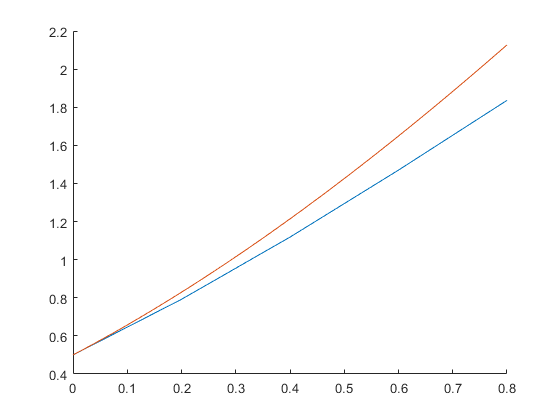
\includegraphics[width=8cm]{Euler/Euler102}
    \centering
    \caption{Resultado del ejercicio 1 con \(h = 0.2\)}\label{fig:euler-1-0-2}
\end{figure}

Si disminuimos el valor de \(h\), se observa como la aproximación converge
a la función original.

\begin{table}[H]
    \begin{center}
        \begin{tabular}{ |c|c|c|c|c| }
            \hline
            Índice & Punto & Valor aproximado & Valor real & Error relativo \\
            \hline
            \hline
            1      & 0     & 0.5              & 0.5        & 0              \\
            \hline
            2      & 0.1   & 0.649            & 0.65741    & 0.012799       \\
            \hline
            3      & 0.2   & 0.8099           & 0.8293     & 0.023392       \\
            \hline
            4      & 0.3   & 0.98189          & 1.0151     & 0.032688       \\
            \hline
            5      & 0.4   & 1.1641           & 1.2141     & 0.04119        \\
            \hline
            6      & 0.5   & 1.3555           & 1.4256     & 0.049208       \\
            \hline
            7      & 0.6   & 1.555            & 1.6489     & 0.056949       \\
            \hline
            8      & 0.7   & 1.7615           & 1.8831     & 0.064565       \\
            \hline
            9      & 0.8   & 1.9737           & 2.1272     & 0.072177       \\
            \hline
            10     & 0.9   & 2.1901           & 2.3802     & 0.079882       \\
            \hline
        \end{tabular}
    \end{center}
    \caption{Tabla del ejercicio 1 con \(h = 0.1\)}\label{tab:euler-1-0-1}
\end{table}

\begin{figure}[H]
    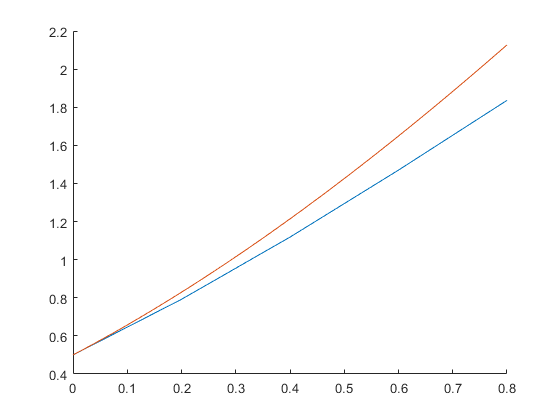
\includegraphics[width=8cm]{Euler/Euler102}
    \centering
    \caption{Resultado del ejercicio 1 con \(h = 0.1\)}\label{fig:euler-1-0-1}
\end{figure}

\begin{table}[H]
    \begin{center}
        \begin{tabular}{ |c|c|c|c|c| }
            \hline
            Índice & Punto  & Valor aproximado & Valor real & Error relativo \\
            \hline
            \hline
            1      & 0      & 0.5              & 0.5        & 0              \\
            \hline
            2      & 0.01   & 0.515            & 0.51507    & 0.00014739     \\
            \hline
            3      & 0.02   & 0.53014          & 0.5303     & 0.00029104     \\
            \hline
            4      & 0.03   & 0.54544          & 0.54567    & 0.0004312      \\
            \hline
            5      & 0.04   & 0.56088          & 0.56119    & 0.00056807     \\
            \hline
            6      & 0.05   & 0.57646          & 0.57686    & 0.00070186     \\
            \hline
            \ldots & \ldots & \ldots           & \ldots     & \ldots         \\
            \hline
            96     & 0.95   & 2.4874           & 2.5096     & 0.0088767      \\
            \hline
            97     & 0.96   & 2.513            & 2.5358     & 0.0089624      \\
            \hline
            98     & 0.97   & 2.5387           & 2.5619     & 0.0090483      \\
            \hline
            99     & 0.98   & 2.5645           & 2.5882     & 0.0091345      \\
            \hline
            100    & 0.99   & 2.5904           & 2.6145     & 0.0092211      \\
            \hline
        \end{tabular}
    \end{center}
    \caption{Tabla del ejercicio 1 con \(h = 0.01\)}\label{tab:euler-1-0-0-1}
\end{table}

\begin{figure}[H]
    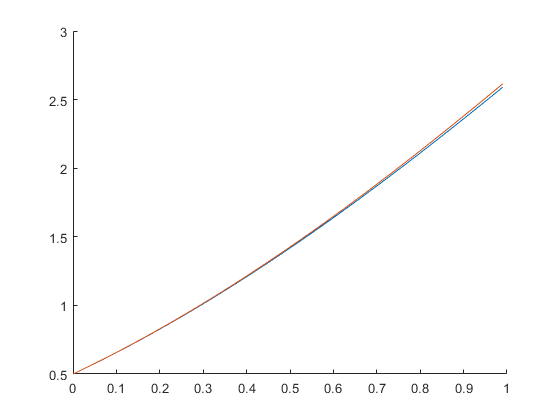
\includegraphics[width=8cm]{Euler/Euler1001}
    \centering
    \caption{Resultado del ejercicio 1 con \(h = 0.01\)}\label{fig:euler-1-0-0-1}
\end{figure}

\subsection{Problema 2}\label{subsec:problema-2}

En el segundo problema se debe resolver el siguiente problema diferencial de Cauchy de
orden 2 por el método de Euler explícito con \(h = 0.05\) y \(T = 0.1\):

\[
    \begin{cases}
        Mu'' = B|u'|u' + ku \quad 0 < t < T \\
        u(0) = u_0
        u'(0) = u_{p0}
    \end{cases}
\]

Se deben usar las constantes \(M = 10 kg\), \(B = 50 Ns^2/m^2\), \(k = 200 N/m\),
\(u_0 = 0\) y \(u_{p0} = 1 m/s\).

Al ser \(h = 0.05\) y \(T = 0.1\), el programa solo ha de integrar una única vez
en el punto \(x = 0.05\).
La gráfica resultante es la siguiente:

\begin{figure}[H]
    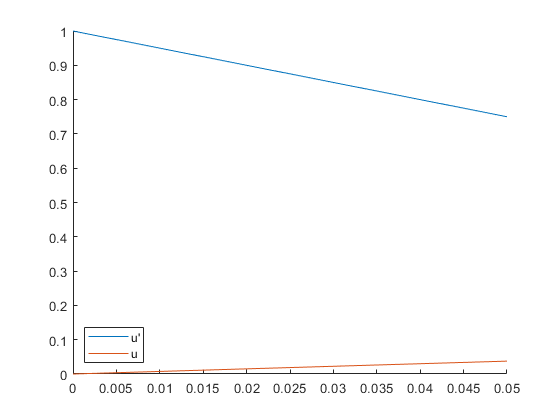
\includegraphics[width=8cm]{Euler/Euler2}
    \centering
    \caption{Resultado del ejercicio 2}\label{fig:euler-2}
\end{figure}

Las variables que más influyen en la ecuación son \(M\) y \(B\).
Si se disminuye el valor de \(M\) y se aumenta el valor de \(B\)
el valor de \(u'\) disminuye considerablemente.

\begin{figure}[H]
    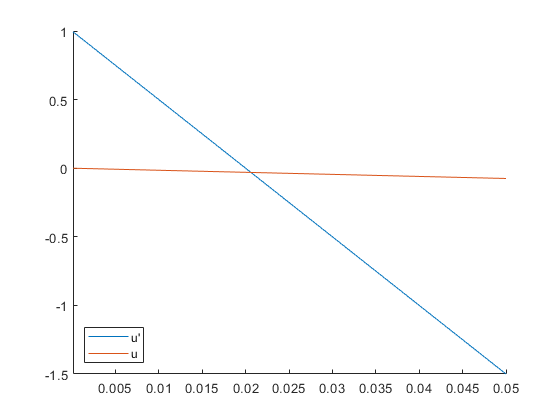
\includegraphics[width=8cm]{Euler/Euler22}
    \centering
    \caption{Resultado del ejercicio 2 con \(M\) disminuido y \(B\) aumentado}
    \label{fig:euler-22}
\end{figure}

